C++中内存管理是要付出代价的。开发者经常抱怨C++需要手动进行内存管理。像C\#和Java这样的语言可以自动内存管理,但程序运行得要比C++程序慢,而手动内存管理通常容易出错且不安全。正如前几章了解到的,程序是数据和指令的集合。几乎每个程序都在某种程度上使用计算机内存,没有一个程序不需要内存分配。 \par
内存分配和回收从最简单的函数调用开始。调用函数通常意味着向它传递参数,函数需要空间来存储这些参数。当代码中声明对象时,会进行自动分配,它们的生存期取决于作用域。只要超出了作用域,就会自动回收它们。大多数编程语言都为动态内存提供了类似的自动回收功能。动态分配内存——与自动分配相反——是开发者根据需要请求新内存的代码部分。例如,当客户数量增加时,将用于存储客户对新内存空间的请求列表到程序中。为了区分不同类型的内存管理,不管是自动的还是手动,开发者使用的都是内存分段。一个程序使用几个内存段、堆栈、堆、只读段等进行操作,尽管它们都具有相同的结构,并且都是虚拟内存的一部分。 \par
大多数语言都提供了访问动态内存的方法,而不关心回收策略,将困难的工作留给运行时环境,C++开发者必须处理内存管理的底层细节。时至今日,C++还是没有提供高级的内存管理功能。因此,对内存结构及其管理的深刻理解是每个C++开发者必须的。这一章中阐明内存背后的奥秘,以及正确的内存管理技术。 \par
本章中,我们将了解以下内容: \par

\begin{itemize}
	\item 什么是内存,C++中如何访问?
	\item 详细的内存分配
	\item 内存管理技术和习惯用法
	\item 垃圾收集的基础
\end{itemize}

\noindent\textbf{}\ \par
\textbf{编译器要求} \ \par
g++编译器需要添加编译选项 \texttt{-std=c++2a} 来编译本章的代码。可以从这里获取本章的源码文件:https:/​/github.​com/PacktPublishing/Expert-CPP \par

\noindent\textbf{}\ \par
\textbf{理解计算机内存} \ \par
底层上理解,存储器是一种存储位的状态的设备。假设我们正在发明一种可以存储单个比特信息的设备,发明很久以前就已经发明了的东西是没有意义的。但它的神奇之处在于,现在的开发者拥有稳定的多功能环境,提供了大量的库、框架和工具来创建程序,甚至不需要理解它们。声明一个变量或分配一个动态内存变得非常容易,如下面的代码片段所示: \par

\begin{lstlisting}[caption={}]
int var;
double* pd = new double(4.2);
\end{lstlisting}

很难描述设备如何存储这些变量。为了解释这个过程,让我们试着设计一个可以存储信息的设备。 \par

\noindent\textbf{}\ \par
\textbf{内存存储的设计} \ \par
我们使用电路、继电器和逻辑门来设计能够进行存储的简单设备。本节的目的是了解内存底层的结构。 \par
这是一个简单的电路图,你们可能在物理课上见过: \par

\begin{center}
	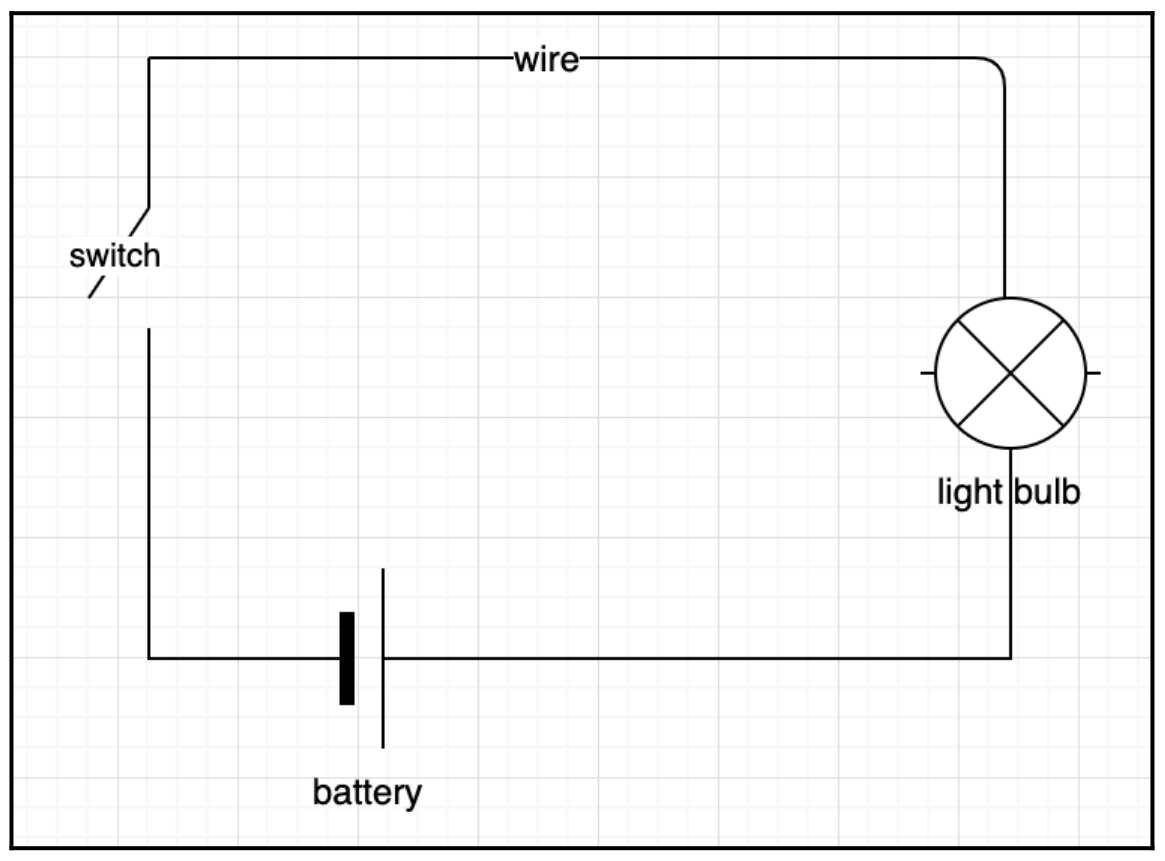
\includegraphics[width=0.6\textwidth]{content/Section-1/Chapter-5/1}
\end{center}

它由一根连接电池和灯泡的电线组成。这根电线上有一个开关,控制灯泡的状态。当开关闭合时,灯泡是亮的,否则是关的。我们将在这个电路中加入两个逻辑非元件,NOR是Not OR的缩写。它通常是这样表示的: \par

\begin{center}
	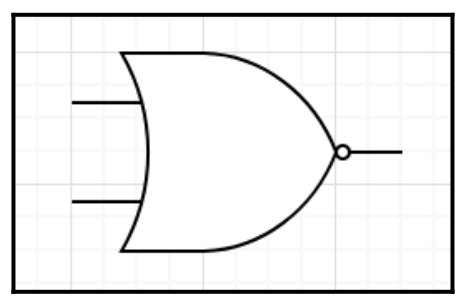
\includegraphics[width=0.2\textwidth]{content/Section-1/Chapter-5/2}
\end{center}

它有两个输入(连接元件的导线),每一个都代表一个电子信号。我们说,如果两个输入都是0,那么输出(从元素出来的导线)是1,这就是为什么我们称它为Not。如果有输入为1,那么OR元素的输出是1。前面的NOR元素简单地使用两个继电器构造。继电器是一种使用电磁铁来闭合和打开触点的开关。请看下图: \par

\begin{center}
	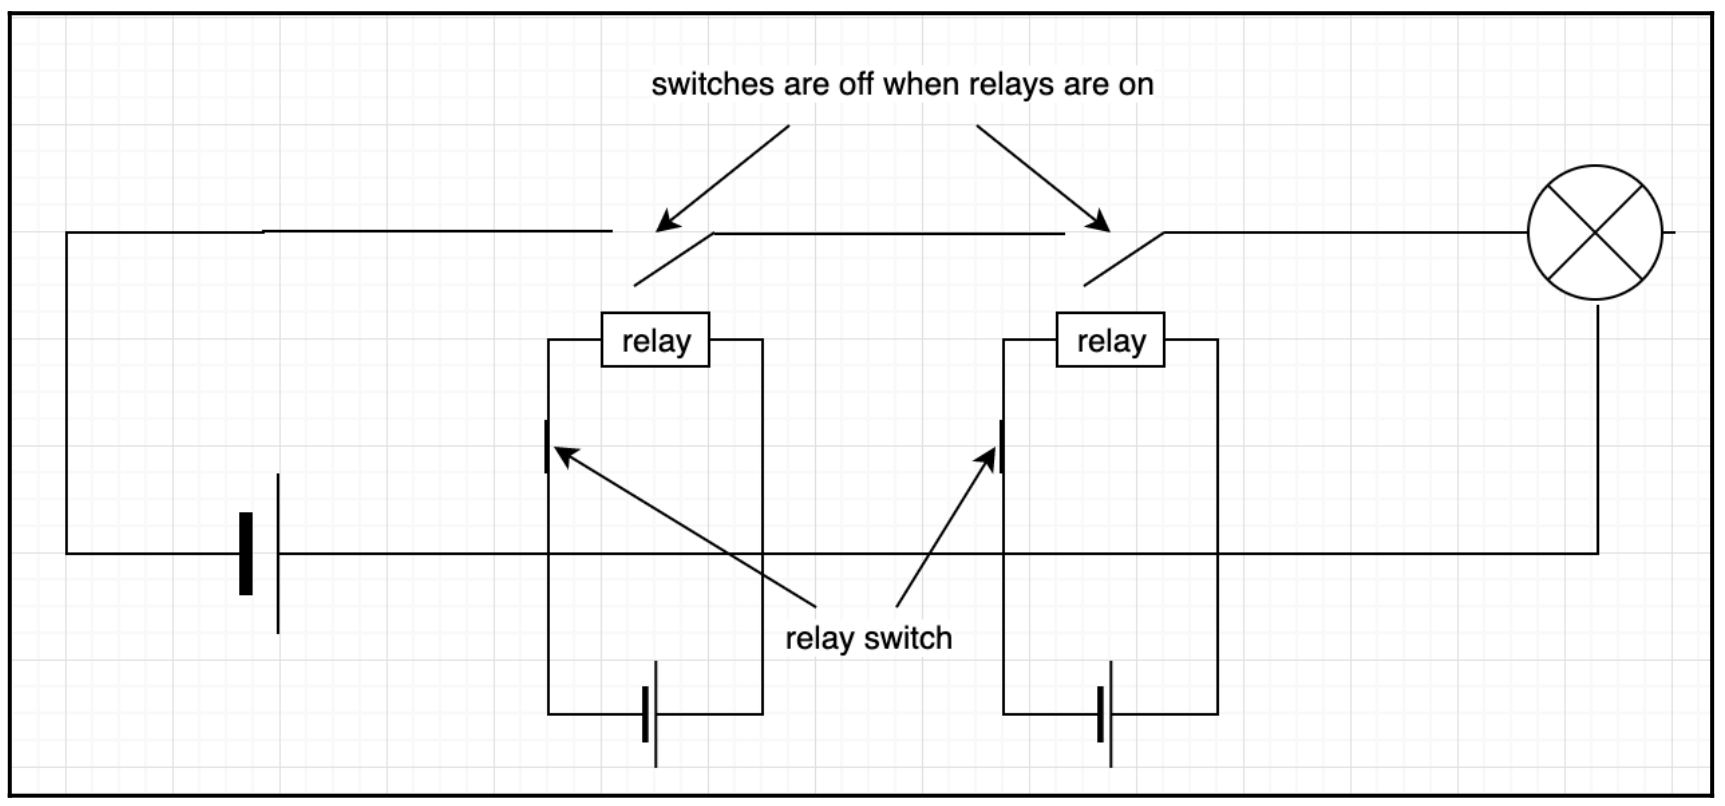
\includegraphics[width=0.6\textwidth]{content/Section-1/Chapter-5/3}
\end{center}

当两个继电器的开关都合上时(即继电器正在工作,并拉下电路的开关),灯泡就灭了。当我们将开关移动到两个继电器的开位时,灯泡就亮了。上图是描述NOR门的一种方法。现在,我们可以使用电线、灯泡、电池和继电器创建逻辑元素。现在让我们来看看两个NOR元素的奇怪组合会导致一个有趣的发现: \par

\begin{center}
	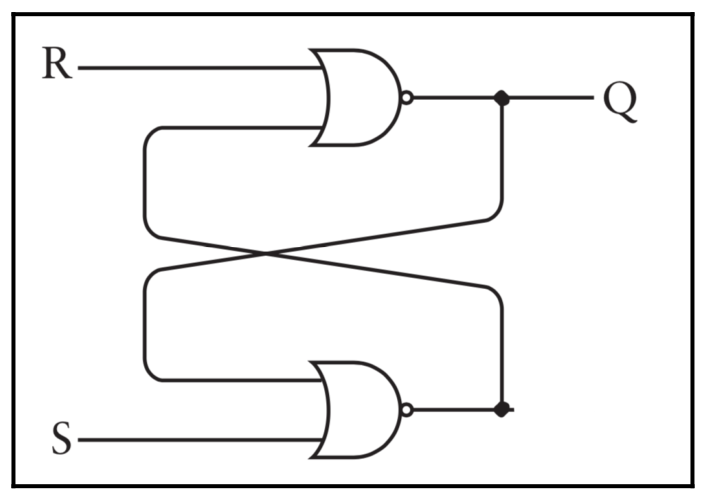
\includegraphics[width=0.4\textwidth]{content/Section-1/Chapter-5/4}
\end{center}

上图是R-S触发器的经典表示。R代表reset, S代表set。按照上述方案构建的设备只能存储1位。输出Q是读取设备内容的连接线。如果我们将触发器设置为存储该位,则输出为1。仔细检查这个图,想象一个个地传递信号给它的输入端,或者同时将信号传递给两个输入端,并看到Q处的输出。当输入S为1时,Q变为1。当R = 1 Q = 0。通过这种方式,我们可以设置或重置位。只要给设备供电,它就会储存数据。 \par
想象一下,有很多早期设计的设备连接在一起,就可以存储不止很多信息。通过这种方式,我们可以构造复杂的存储设备,来存储字节甚至千字节的数据。 \par
前面的设备与晶体管发明之前的计算机中使用的设备相似。晶体管是一种存储量小得多的设备。现代设备不使用继电器,而是结合了数百万个晶体管来存储和操作数据。中央处理单元(CPU)寄存器是一种利用晶体管来存储特定数量位元的设备。通常,一个通用寄存器最多存储64位数据。不仅能使用寄存器来存储所有的程序和数据,现代计算机的内存结构要复杂得多。现在,让我们从更的角度来研究计算机内存的层次结构。 \par

\noindent\textbf{}\ \par
\textbf{从更高层次的角度理解计算机内存} \ \par

编写专业程序时,了解计算机内存和数据存储的细节至关重要。当开发者提到内存时,大多数指的是虚拟内存。虚拟内存是操作系统(OS)支持的一种抽象内存,它控制并为进程提供内存空间。每个进程都有它的地址空间表示为几个段的集合。第2章中讨论了内存段的种类,以及给定程序如何使用它们。从开发者的角度来看,访问内存空间主要限于对象声明和使用,无论是堆栈、堆还是静态内存上声明对象,都访问相同的内存抽象——虚拟内存,直接使用物理内存比较困难。作为开发者至少应该知道有哪些内存存储单元,以及如何利用这些知识来编写更好的代码。 \par
本节中,讨论了内存层次物理结构,我们称它为层次结构,因为在较低层次的每个内存单元提供更快的访问,但空间小。每一个连续的更高级别的内存提供了更多的空间,但访问速度更慢。讨论物理内存层次结构,有助于我们设计更好的代码。 \par
了解内存在各个层次上的工作原理,有助于开发者更好地组织数据操作。下面的图表说明了内存的层次结构: \par

\begin{center}
	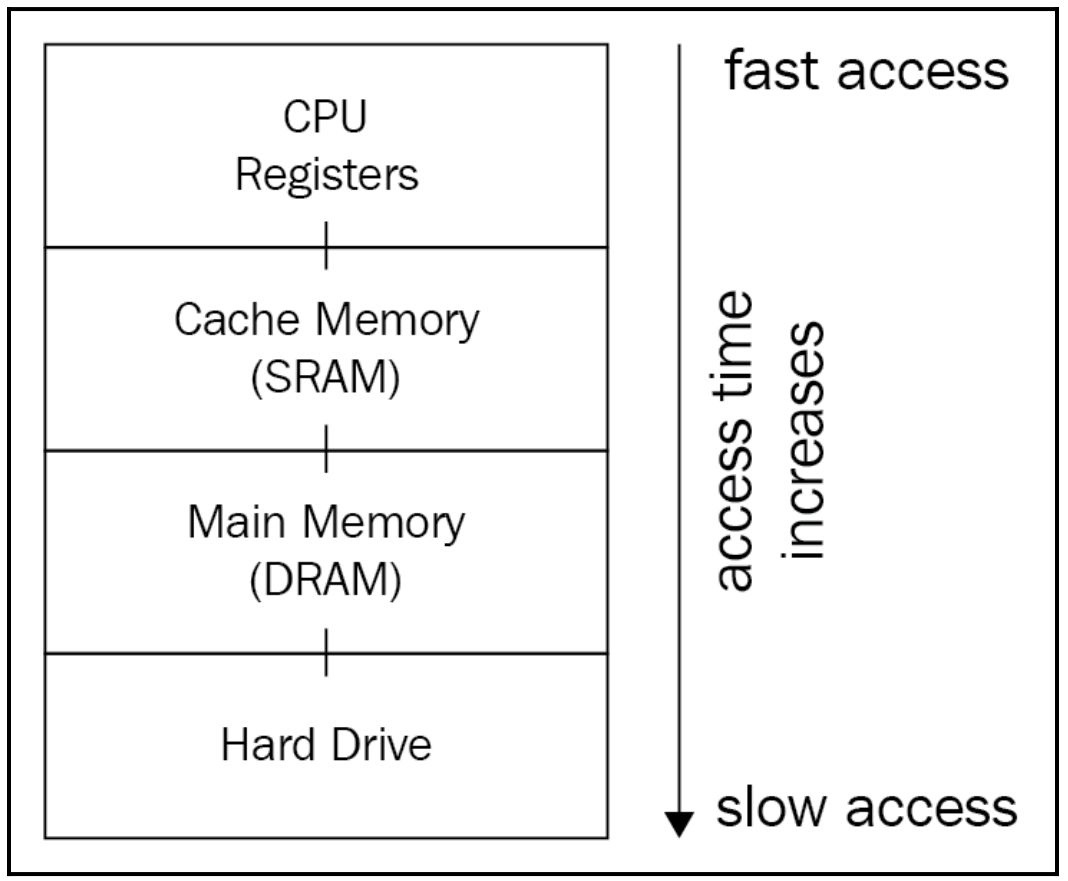
\includegraphics[width=0.6\textwidth]{content/Section-1/Chapter-5/5}
\end{center}

寄存器是放置在中央处理器中的可访问存储器单元。寄存器的数量有限,所以不能把所有的程序数据都保存在里面。另一方面,动态RAM (DRAM)能够为程序存储数据。由于DRAM的物理结构和与CPU之间的距离,需要更长的时间来访问数据。CPU通过数据总线访问DRAM,数据总线是一组在CPU和DRAM之间传输数据的线。为了通知DRAM控制器它将读或写数据,CPU使用控制总线。我们将DRAM称为主存,来详细看看内存层次结构。 \par

\noindent\textbf{}\ \par
\textbf{寄存器} \ \par
寄存器保存固定数量的数据。CPU字大小通常由寄存器的最大长度定义,例如:8个字节或4个字节。C++程序不能直接访问寄存器。 \par

\hspace*{\fill} \\ %插入空行

\includegraphics[width=0.05\textwidth]{images/warn}
C++支持使用asm声明嵌入汇编代码,例如,\texttt{asm("mov edx, 4")}。属于特定于平台的代码,所以不建议使用。\par
\noindent\textbf{}\ \par

在旧版本中,可以在声明变量时使用register关键字: \par

\begin{lstlisting}[caption={}]
register int num = 14;
\end{lstlisting}

修饰符指定编译器将变量存储在寄存器中。这样,它给开发者一种代码被优化的假象。 \par

\hspace*{\fill} \\ %插入空行

\includegraphics[width=0.05\textwidth]{images/tip}
编译器是将高级C++代码转换为机器代码的工具。翻译过程中,代码需要进行多次转换,包括代码优化。当开发者使用技巧使编译器优化部分代码时,编译器会把它们当作建议而不是命令。\par
\noindent\textbf{}\ \par

例如,在循环中访问一个变量,如果该变量放在寄存器中比放在DRAM中要快。例如,下面的循环访问对象一百万次: \par

\begin{lstlisting}[caption={}]
auto number{42};
for (int ix = 0; ix < 10000000; ++ix) {
	int res{number + ix};
	// do something with res
}
\end{lstlisting}

这个数字有一个自动的存储时间(与auto关键字无关),并放置在堆栈上。堆栈是虚拟内存中的一段,而虚拟内存是物理DRAM的抽象。寄存器中访问对象要比在DRAM中快得多,假设从DRAM中读取number的值比从寄存器中读取要慢5倍。使用register关键字优化前面循环的结果是显而易见的,如下所示: \par

\begin{lstlisting}[caption={}]
register auto number{42};
// the loop omitted for code brevity
\end{lstlisting}

然而,现在的编译器可以进行更好的优化,因此随着时间的推移,对修饰符的需求已经消失,现在它已经是弃用的语言特性了。更好的优化方法是完全去掉number对象。 \par
例如,下面的代码代表了编译优化版本,它使用实际的值,而不是通过驻留在DRAM中的变量来访问它: \par

\begin{lstlisting}[caption={}]
for (int ix = 0; ix < 1000000; ++ix) {
	int res{42 + ix};
	// do something with res
}
\end{lstlisting}

虽然前面的例子很简单,但是应该考虑编译过程中发生的编译器优化。 \par
寄存器可以提高我们对程序执行细节的理解,CPU执行的所有操作都通过寄存器进行,包括CPU解码和执行的指令,都是使用特定的寄存器访问,通常称指定执行指令的寄存器为指令指针。当运行程序时,CPU访问它的指令,解码并执行。从主存读取数据和向内存写入数据,通过从寄存器复制数据和向寄存器复制数据来完成。通常,当CPU对数据执行操作时,通用寄存器用来保存数据。下面的图表描述了CPU的抽象视图,以及通过总线与主存储器的交互: \par

\begin{center}
	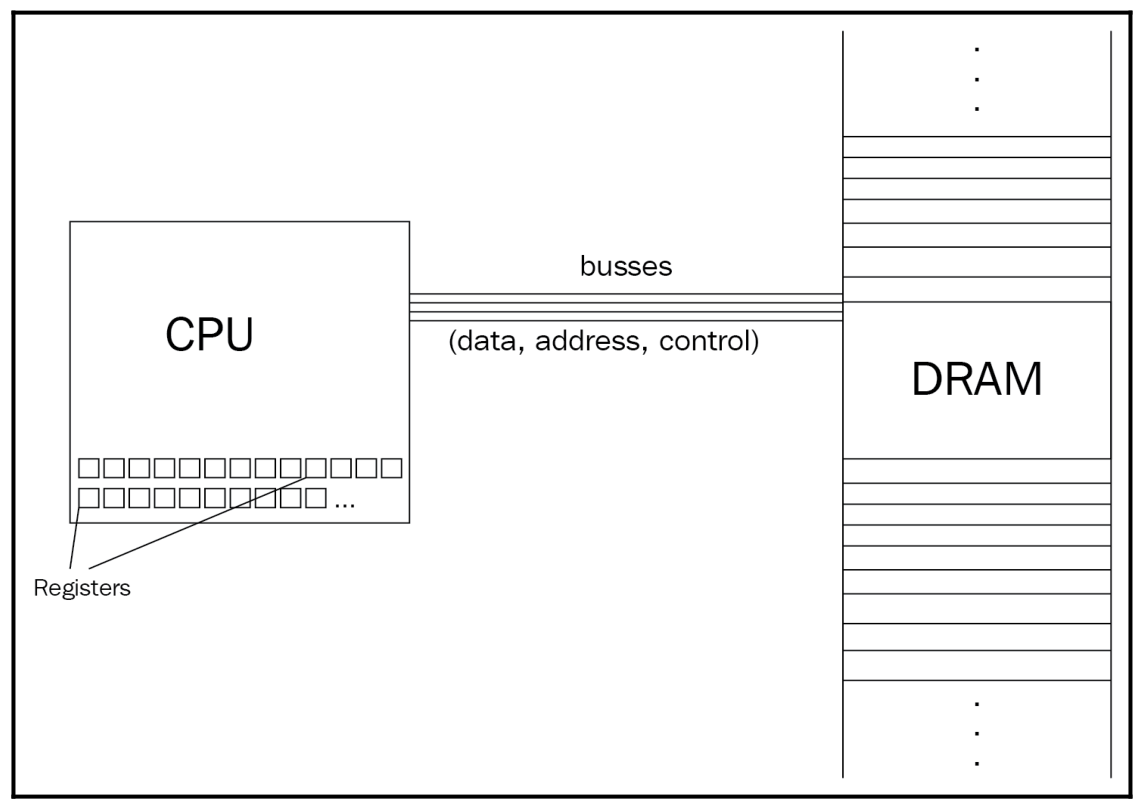
\includegraphics[width=0.6\textwidth]{content/Section-1/Chapter-5/6}
\end{center}

CPU和DRAM之间的通信通过各种总线进行。第2章中用C++进行底层编程时,我们讨论了C++程序的底层表示——应该会看一下,以便更好地理解下面的例子。 \par
现在,让我们看看实际的寄存器。下面的C++代码声明了两个变量,并将它们的和存储在第三个变量中: \par

\begin{lstlisting}[caption={}]
int a{40}, b{2};
int c{a + b};
\end{lstlisting}

为了执行sum指令,CPU将变量a和b的值移动到寄存器中。在计算和之后,将结果移动到另一个寄存器。程序的汇编伪代码表示形式类似于下面的代码: \par

\begin{lstlisting}[caption={}]
mov eax, a
mov ebx, b
add eax, ebx
\end{lstlisting}

编译器并不是必须生成将每个变量映射到寄存器的代码——因为寄存器的数量是有限的。只需要记住,将经常访问的变量保持在足够小的大小,以便能够将其放入其中一个寄存器。对于更大的对象,缓存、内存会起到帮助作用。 \par

\noindent\textbf{}\ \par
\textbf{缓存} \ \par
缓存的概念在编程和计算机系统中很常见。加载在浏览器中的图像可以缓存,以避免将来用户再次访问该网站时向Web服务器请求下载它。缓存使程序运行得更快,这个概念可以以多种形式使用,包括单个功能。例如,下面的递归函数计算阶乘:\par

\begin{lstlisting}[caption={}]
long factorial(long n) {
	if (n <= 1) { return 1; }
	return n * factorial(n - 1);
}
\end{lstlisting}

这个函数不记得它以前计算的值,所以下面的调用会导致5次和6次递归调用: \par

\begin{lstlisting}[caption={}]
factorial(5); // calls factorial(4), which calls factorial(3), and so on
factorial(6); // calls factorial(5), which calls factorial(4), and so on
\end{lstlisting}

可以将已经计算好的值存储在一个全局可访问的变量中,如下所示: \par

\begin{lstlisting}[caption={}]
std::unordered_map<long, long> cache;

long factorial(long n) {
	if (n <= 1) return 1;
	if (cache.contains(n)) return cache[n];
	cache[n] = n * factorial(n - 1);
	return cache[n];
}
\end{lstlisting}

这些修改优化了对该函数的进一步调用: \par

\begin{lstlisting}[caption={}]
factorial(4);
// the next line calls factorial(4), stores the result in cache[5], which
then calls factorial(3)
// and stores the result in cache[4] and so on
factorial(5);
factorial(6); // calls the factorial(5) which returns already calculated
value in cache[5]
\end{lstlisting}

缓存的概念使阶乘函数运行得更快,与此相同的是,名为cache的实际内存设备被放置在CPU中。该设备存储最近访问的数据,以便进一步更快地访问该数据。下面的图表描述了CPU内部的寄存器和缓存内存: \par

\begin{center}
	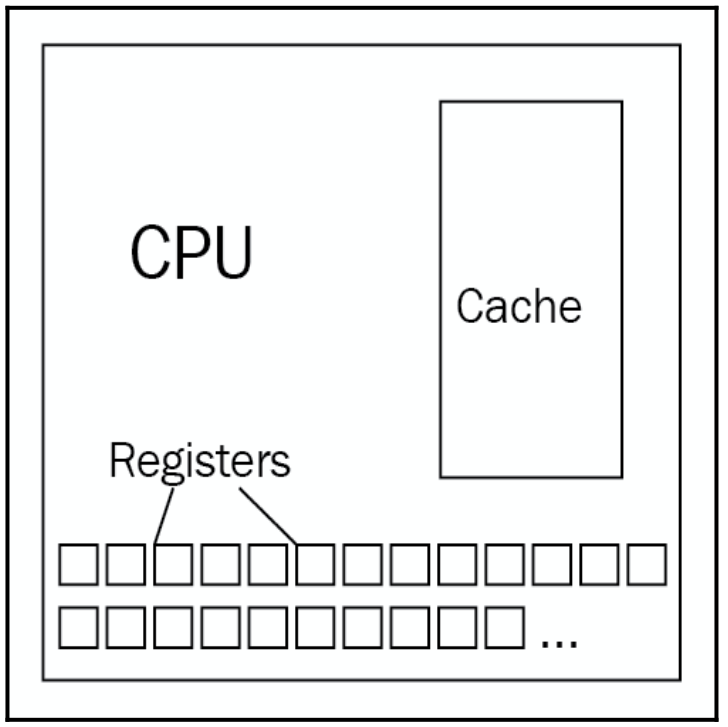
\includegraphics[width=0.6\textwidth]{content/Section-1/Chapter-5/7}
\end{center}

缓存大小通常在2KB到64KB之间(很少是128KB)。虽然对于像Photoshop这样的应用程序来说不够大,因为图像数据的大小可能比缓存本身大得多,但在很多情况下,确实有帮助。例如,假设我们在一个向量中存储了1000多个数字: \par

\begin{lstlisting}[caption={}]
std::vector<int> vec;
vec.push_back(1);
...
vec.push_back(9999);
for (auto it: vec) {
	std::cout << it;
}
// 1
// 2
// 3
// ...
// 9999
\end{lstlisting}

假设要打印该项,CPU将其从内存复制到rax寄存器,然后调用操作符<<,该操作符将rax的值打印到屏幕上。每次迭代循环中,CPU将vector的下一项复制到rax寄存器中,并调用该函数打印其值。每个拷贝操作都要求CPU在地址总线上放置项目的地址,并将控制总线设置为读模式。DRAM微控制器通过地址总线接收到的地址访问数据,并将其值复制到数据总线,从而将数据发送给CPU。CPU将值定向到rax寄存器,然后执行指令打印它的值。下面的图表显示了CPU和DRAM之间的这种交互: \par

\begin{center}
	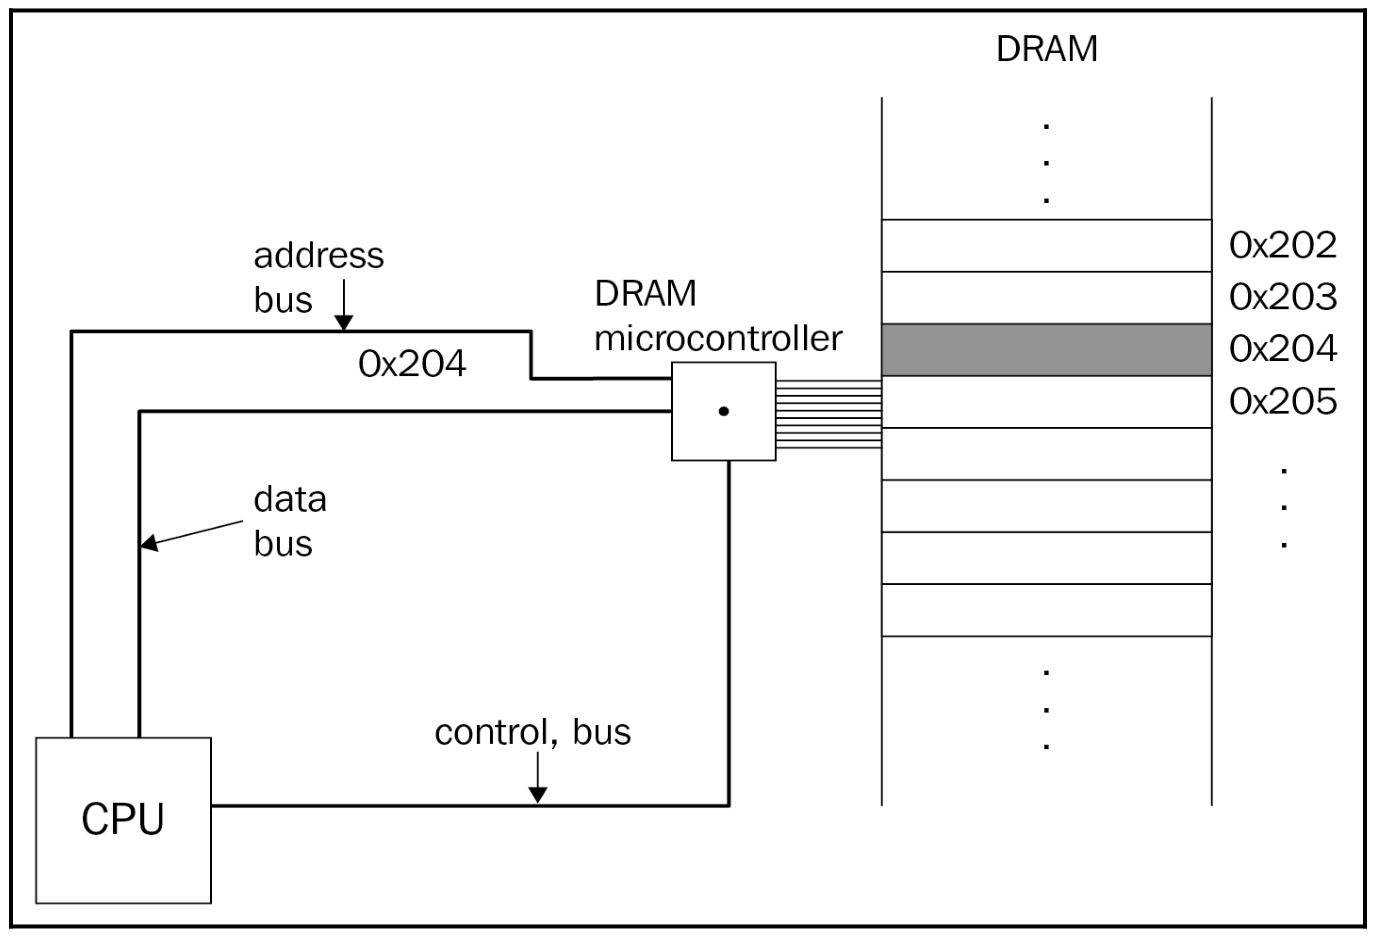
\includegraphics[width=0.6\textwidth]{content/Section-1/Chapter-5/8}
\end{center}

为了优化循环,CPU保持了数据本地化的思想,将整个向量复制到缓存中,并从缓存中访问向量,省略了对DRAM不必要的请求。下面的图表中,你可以看到通过数据总线从DRAM接收到的数据,然后存储在高速缓存存储器中:\par

\begin{center}
	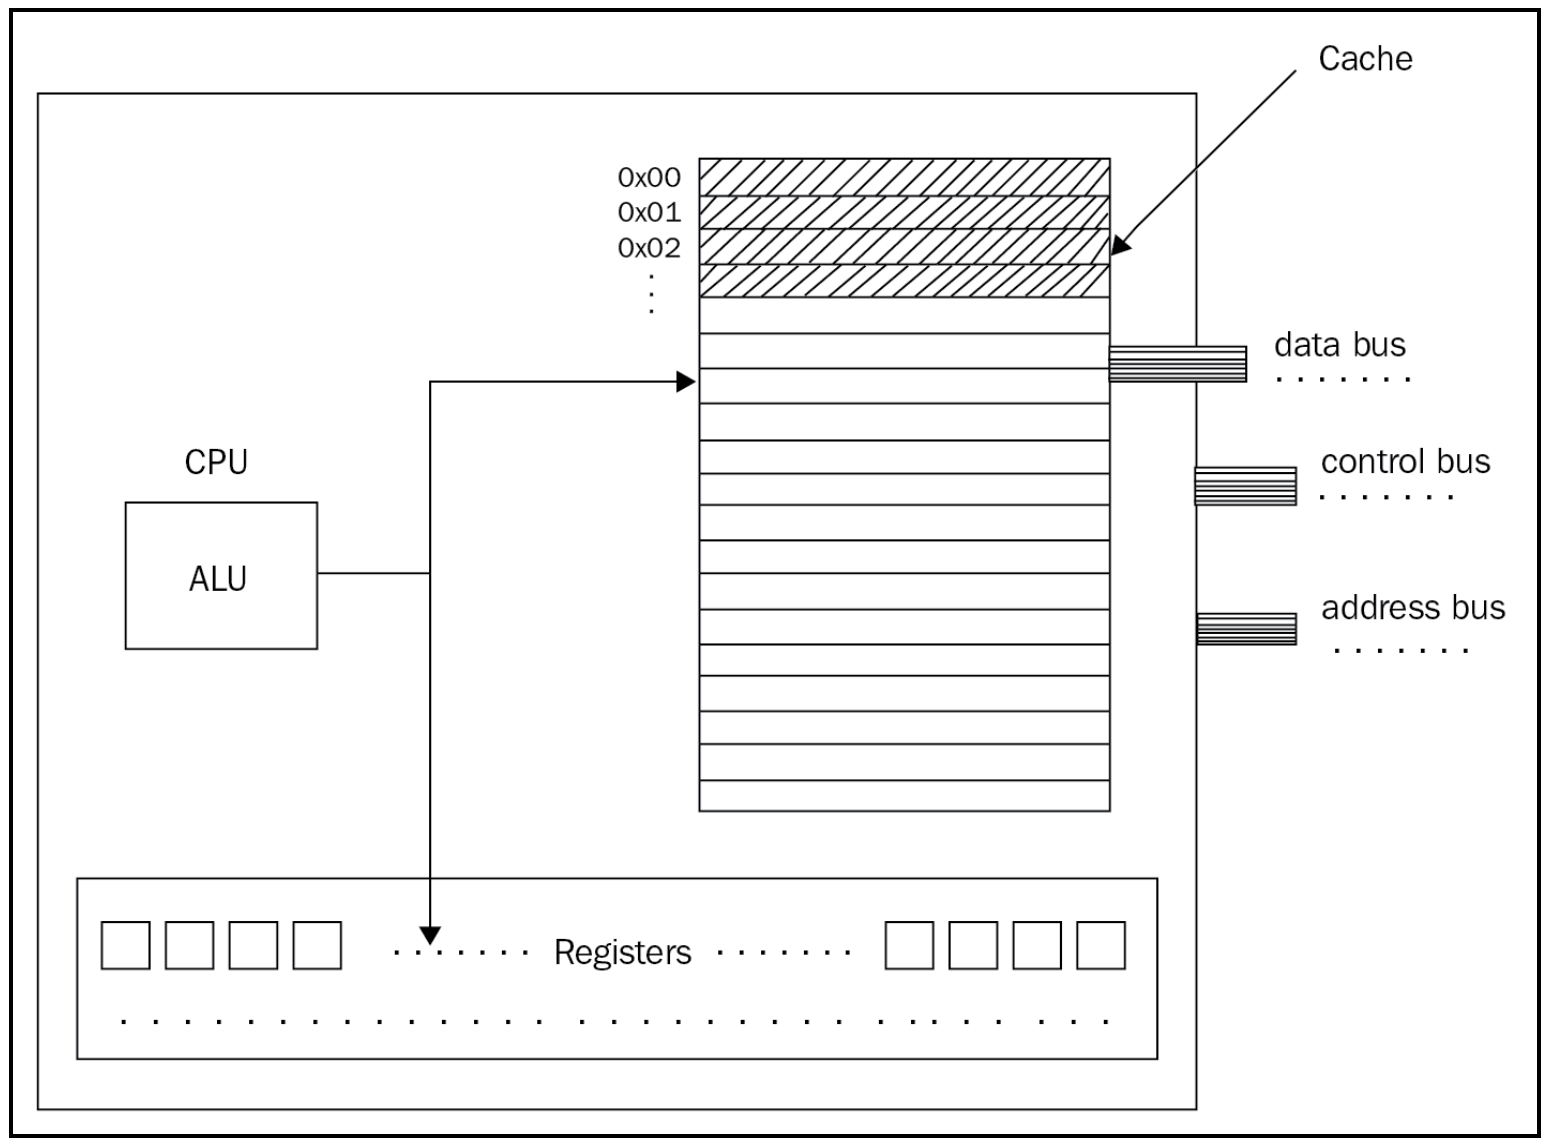
\includegraphics[width=0.6\textwidth]{content/Section-1/Chapter-5/9}
\end{center}

位于CPU中的高速缓存称为一级(L1)高速缓存,它的容量最小,位于CPU内部。许多架构都有2级(L2)缓存,它位于CPU之外(虽然比主存更近),并且以与DRAM相同的方式访问。L2高速缓存和DRAM之间的区别是物理结构和数据访问模式。L2高速缓存代表静态RAM(SRAM),它比DRAM快,但价格更高。 \par

\hspace*{\fill} \\ %插入空行

\includegraphics[width=0.05\textwidth]{images/tip}
一些运行时环境在实现垃圾收集时,会利用缓存的思想。它们根据对象的生存期将对象划分为不同的类别,其中生存期最小的对象(如在代码的局部范围内分配的对象)放置在缓存中,以便更快地访问和释放。 \par
\noindent\textbf{}\ \par

新的缓存内存级别充当较低级别的缓存。例如,L2缓存作为L1缓存的缓存内存。当CPU遇到缓存缺失时,它请求L2缓存,以此类推。 \par

\noindent\textbf{}\ \par
\textbf{主存} \ \par
DRAM的物理结构迫使它以刷新电荷以保持数据稳定,而SRAM不需要像DRAM那样刷新。我们称DRAM为主存主要是因为程序被装入其中,操作系统维护虚拟内存可以映射到DRAM中。所有实际的工作首先通过主存进行。 \par
主内存表示可寻址的数据字节序列。每个字节都有唯一地址,并使用该地址访问。前面提到过CPU如何在地址总线上放置数据的地址,从而让DRAM控制器获取请求的数据并通过数据总线发送它。 \par
操作系统引入虚拟内存作为物理内存的抽象,将虚拟内存的内容映射到物理内存,这涉及到CPU的译后备用缓冲区(TLB)。TLB是另一种形式的缓存内存:它存储虚拟内存到物理内存的最近转换,因此缓存它以备将来的请求。如下图所示,CPU与TLB协调,以便将虚拟地址转换为正确地物理地址 :\par

\begin{center}
	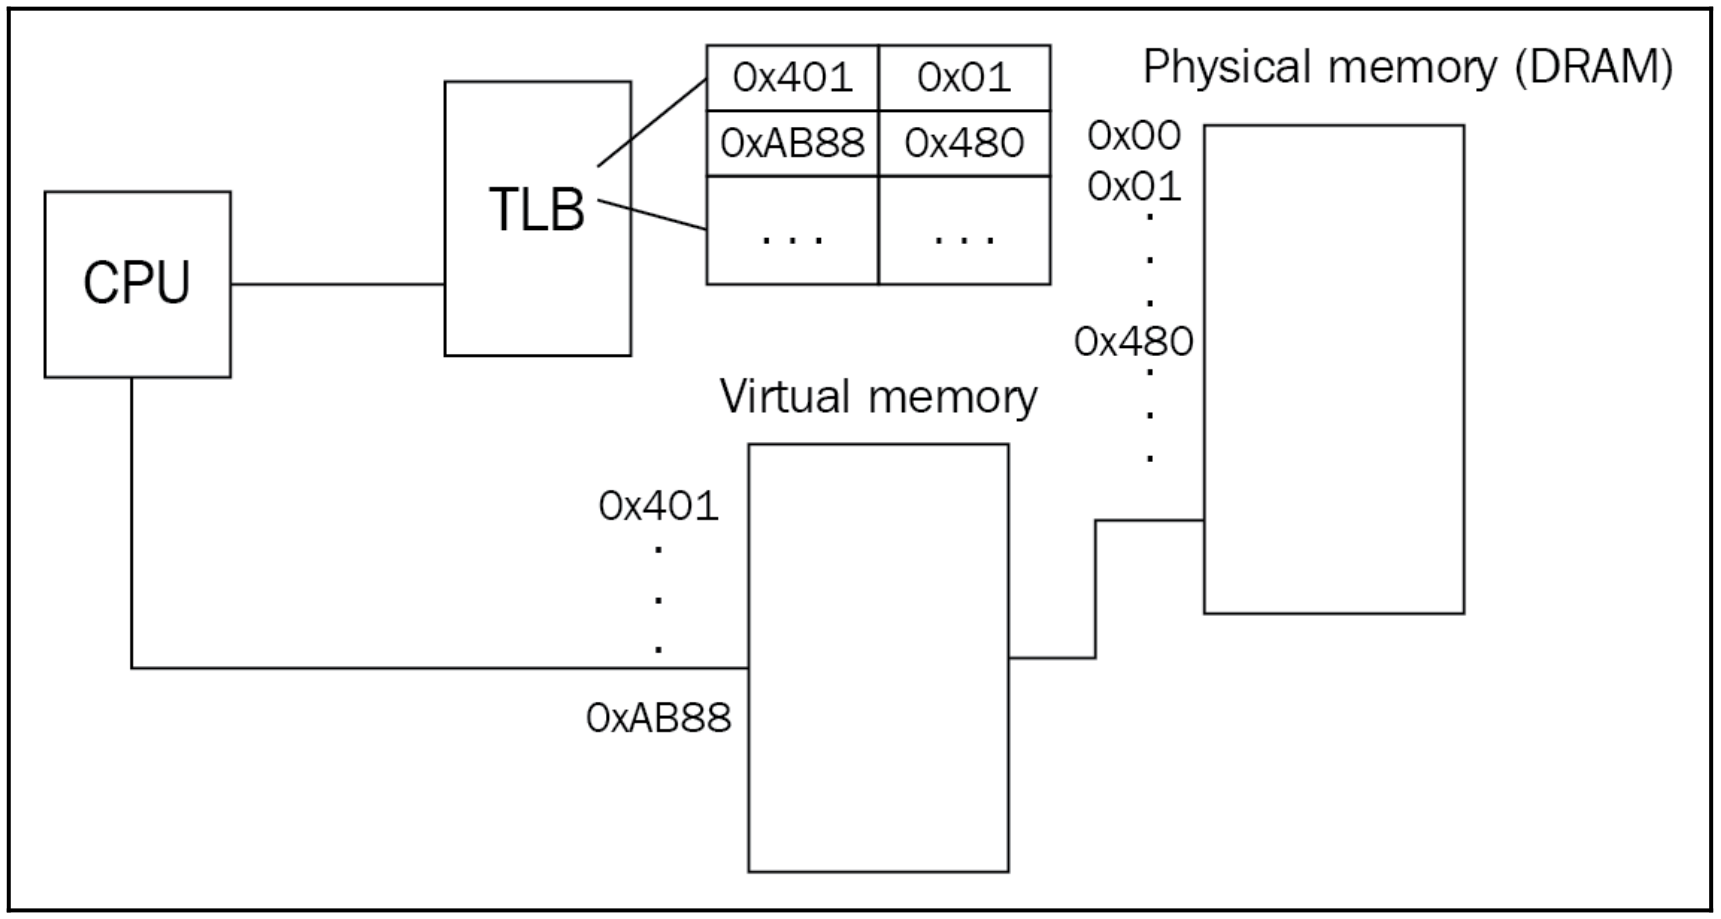
\includegraphics[width=0.6\textwidth]{content/Section-1/Chapter-5/10}
\end{center}

尽管内存管理很复杂,但操作系统为我们提供了一个足够简单的抽象来管理程序所需的内存。我们可以使用堆栈自动分配它,也可以在堆上动态分配。自动内存分配实际上不涉及很多问题和困难,我们只是声明对象,然后将它们放在堆栈上,然后在执行离开作用域时自动删除。动态内存的情况下(不要与前面提到的硬件DRAM混淆),分配和回收都应该手动完成,这可能会导致导致内存泄漏。 \par

\noindent\textbf{}\ \par
\textbf{固定存储器} \ \par
当我们关闭计算机时,主存储器的内容将被删除(因为电荷不再刷新)。为了在断电的情况下永久存储数据,计算机配备了硬盘驱动器(HDD)或固态驱动器(SSD)。从开发者的角度来看,永久存储是用来存储程序所需的数据。为了运行一个程序,它应该加载到主存储器——从硬盘复制到DRAM。操作系统使用加载程序处理它,并在内存中创建一个程序映像,称为进程。当程序完成或用户关闭它时,操作系统将进程的地址范围标记为可自由使用。 \par
我们假设在学习C++的时候使用一个文本编辑器来写笔记。输入到编辑器中的文本驻留在主存中,除非我们将其保存在硬盘上。注意这一点很重要,因为大多数程序都会跟踪用户最近的活动,并且允许用户修改程序设置。为了保持这些设置,即使在程序重新启动后,用户修改他们的方式,程序将他们作为一个单独文件存储在硬盘上。程序下次运行时,首先从硬盘读取相应的设置文件,并更新自己以应用最近的设置。 \par
通常,永久存储比主存有更大的容量,这使得可以使用硬盘驱动器作为虚拟内存的备份。操作系统可以维持虚拟内存并伪造其大小,使其比物理DRAM更大。例如,通过启动几个重量级应用程序,DRAM的最大容量可能会很快耗尽。然而,操作系统仍然可以通过备份硬盘上的额外空间来维持更大的虚拟内存。当用户在应用程序之间切换时,操作系统将超出的虚拟内存字节复制到硬盘,并将当前运行的应用程序映射到物理内存。 \par
这使得程序和操作系统运行得更慢,但允许我们在不考虑主存有限大小的情况下保持它们的打开状态。现在让我们更深入地研究一下C++中的内存管理。 \par

\noindent\textbf{}\ \par
\textbf{内存管理的基础知识} \ \par
大多数情况下,当开发者忘记重新分配内存空间时,内存管理中出现的问题就会发生。这将导致内存泄漏。内存泄漏在程序中都是普遍存在的问题。当程序为其数据请求一个新的内存空间时,操作系统将提供的空间标记为busy,该程序的其他指令或任何其他程序都不能请求那么多内存空间。理想情况下,当程序的部分使用完内存空间后,必须通知操作系统删除busy标签,以使该空间可供其他程序使用。有些语言提供了对动态分配内存的自动控制,这样就能开发者专注于程序的逻辑,而不是关注内存资源的回收。然而,C++假设开发者是负责的(通常不是这样),动态分配的内存管理是开发者的职责。这就是为什么该语言同时提供了new和delete操作符来处理内存空间,其中new操作符分配内存空间,delete操作符释放内存空间。换句话说,处理动态分配内存的理想代码如下所示: \par

\begin{lstlisting}[caption={}]
T* p = new T(); // allocate memory space
p->do_something(); // use the space to do something useful
delete p; // deallocate memory space
\end{lstlisting}

忘记调用delete操作符会使分配的内存空间永远处于busy状态。现在想象一个始终在用户计算机上打开的Web浏览器。随着时间的推移,内存泄漏可能会导致内存不足,用户迟早需要重新启动程序,或者重启操作系统。 \par
这个问题适用于使用的任何资源,无论是文件还是忘记关闭的套接字(更多关于套接字的内容,请参阅第12章)。为了解决这个问题,C++开发者使用了资源获取即初始化(RAII)的习惯用法,在获得资源时初始化,适当时释放资源。让我们看看它的实际应用。 \par

\noindent\textbf{}\ \par
\textbf{内存管理的例子} \ \par
考虑以下函数,动态分配一个包含420个short的数组,从用户输入中读取它们的值,按升序打印它们,然后释放数组: \par

\begin{lstlisting}[caption={}]
void print_sorted() {
	short* arr{new short[420]};
	for (int ix = 0; ix < 420; ++ix) {
		td::cin >> arr[ix];
	}
	std::sort(arr, arr + 420);
	for (int ix = 0; ix < 420; ++ix) {
		std::cout << arr[ix];
	}
	delete arr; // very bad!
}
\end{lstlisting}

前面的代码中,我们已经犯了一个错误,使用了错误的delete操作符来释放内存。要释放数组,必须使用delete[]操作符,否则代码会导致内存泄漏。下面是我们如何演示数组的分配: \par

\begin{center}
	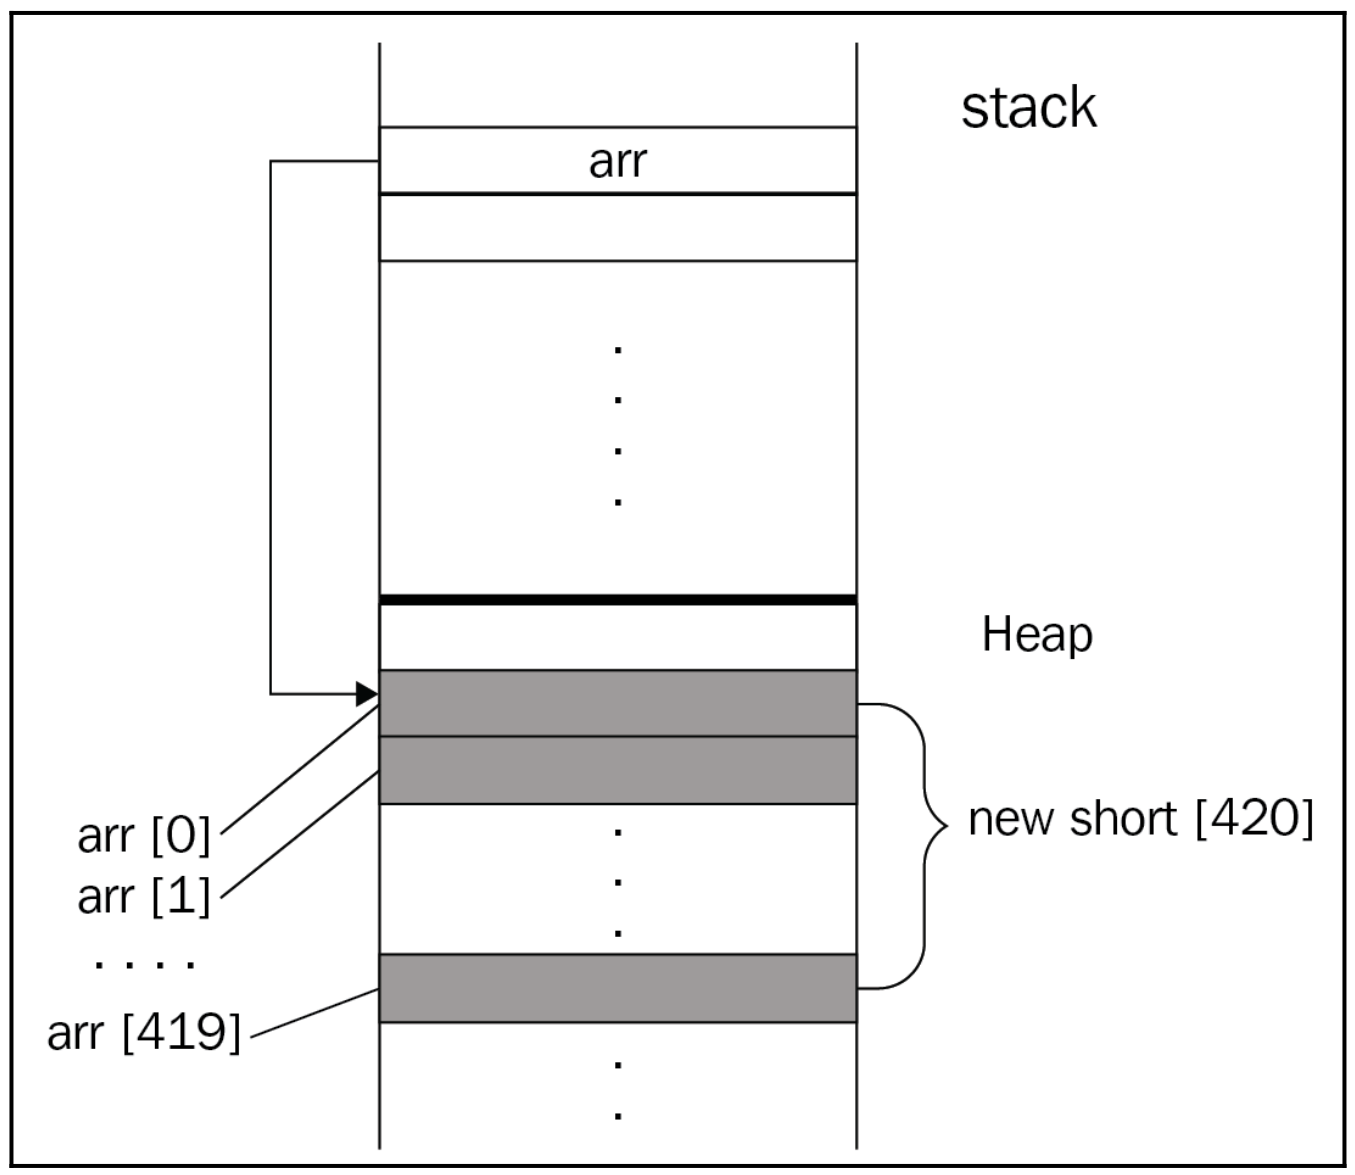
\includegraphics[width=0.6\textwidth]{content/Section-1/Chapter-5/11}
\end{center}

假设我们使用delete而不是delete[]来释放空间。它将把arr作为一个短指针来处理,因此将删除从arr指针中包含的地址开始的前两个字节,如下图所示: \par

\begin{center}
	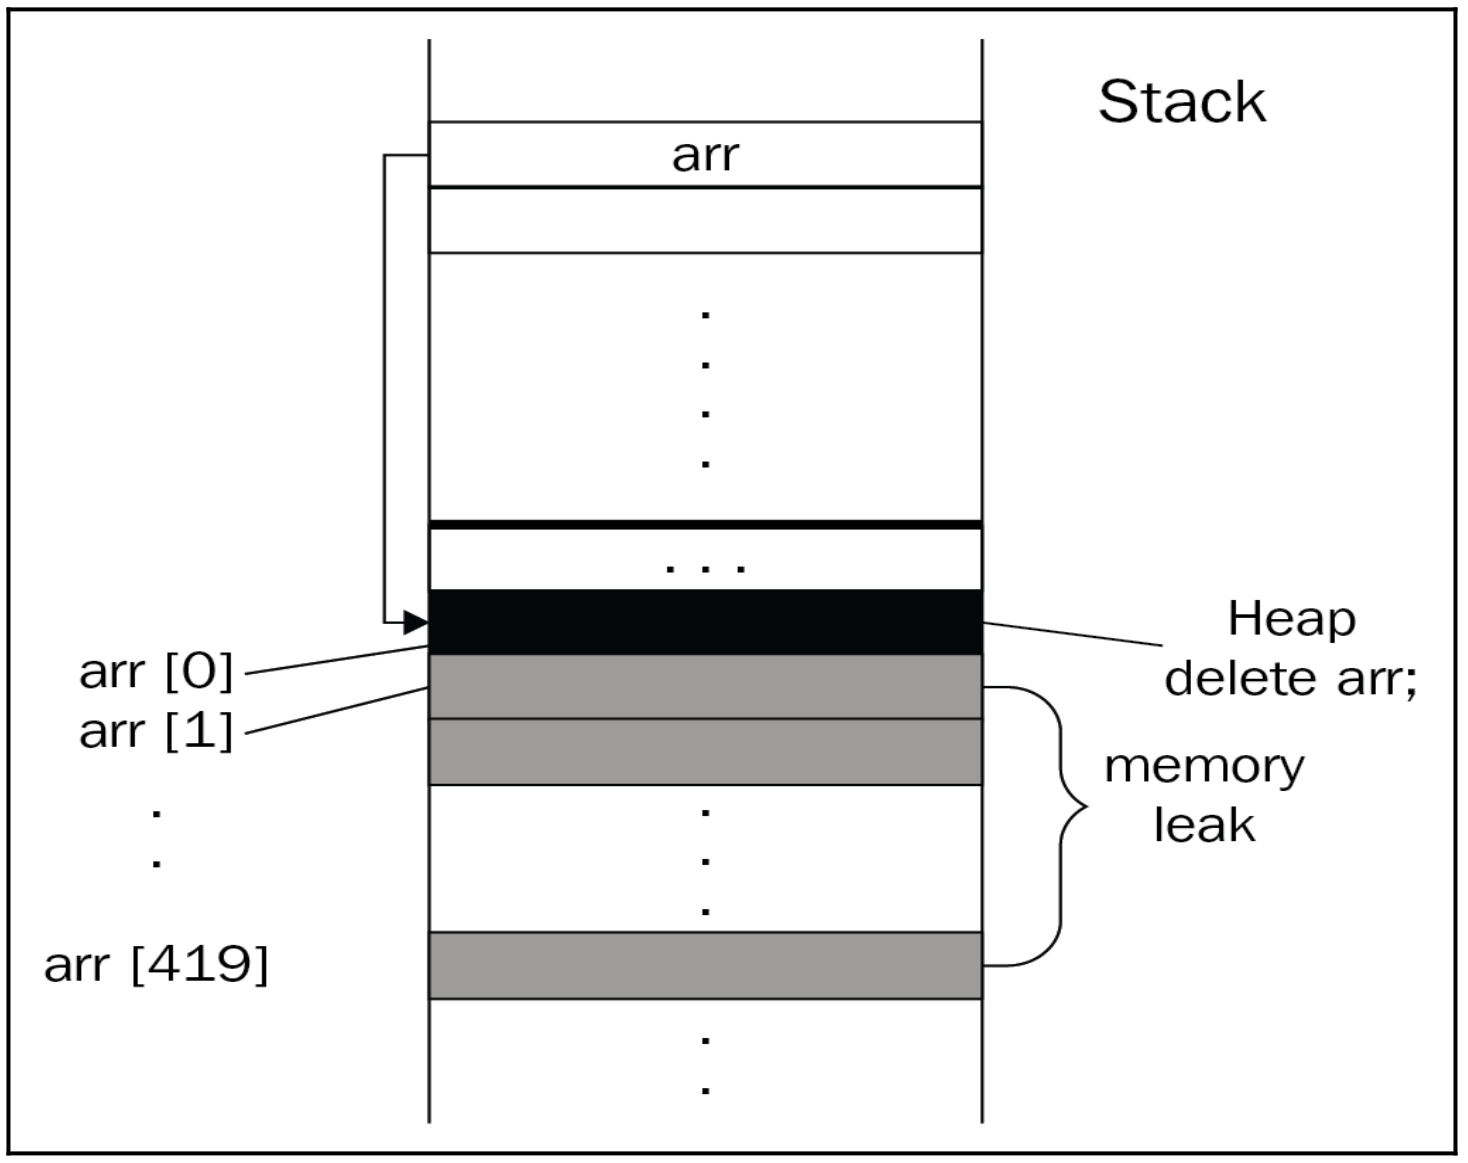
\includegraphics[width=0.6\textwidth]{content/Section-1/Chapter-5/12}
\end{center}

所以现在我们从420个中移除第一个,并让419个shoet保持原样。当我们在堆上需要新的空间时,包含419个不可接触对象的那部分将不会再重用。尽管new和delete操作符族是由实现定义的,但我们不应该奢望以这种方式避免内存泄漏。 \par
让我们修改前面的代码,以正确释放为数组分配的内存,并确保消除了输入负数的可能: \par

\begin{lstlisting}[caption={}]
void print_sorted() {
	short* arr{new short[420]};
	for (int ix = 0; ix < 420; ++ix) {
		std::cin >> arr[ix];
		if (arr[ix] < 0) return;
	}
	std::sort(arr, arr + 420);
	// print the sorted array, code omitted for brevity
	delete[] arr;
}
\end{lstlisting}

前面的修改是可能的内存泄漏的另一个例子,不过为了简单起见,我们编写了难看的代码。只要用户输入一个负数,函数就返回。这就给我们留下了420个孤儿short。然而,对分配的内存的唯一访问是arr指针,它是在堆栈上声明的,因此当函数返回时,它将自动删除(指针变量,而不是指向它的内存空间)。为了消除内存泄漏的可能性,只需在函数退出之前使用delete[]操作符: \par

\begin{lstlisting}[caption={}]
void print_sorted() {
	short* arr{new short[420]};
	for(int ix = 0; ix < 420; ++ix) {
		std::cin >> arr[ix];
		if (arr[ix] < 0) {
			delete[] arr;
			return;
		}
	}
	// sort and print the sorted array, code omitted for brevity
	delete[] arr;
}
\end{lstlisting}

代码变得有些难看,但它修复了内存泄漏。如果进一步修改该函数,并使用第三方标准库函数对数组进行排序,会怎么样呢? \par

\begin{lstlisting}[caption={}]
import <strange_sort.h>;
void print_sorted() {
	short* arr{new short[420]};
	for (...) { /* code omitted for brevity */ }
	strange_sort::sort(arr, arr + 420);
	// print the sorted array, code omitted for brevity
	delete[] arr;
}
\end{lstlisting}

结果是,当数组项的值超过420时,strange\underline{ }sort::sort会抛出异常(这就是为什么它是一个奇怪的排序)。如果异常未被捕获,将使用冒泡排序的函数,除非它在某个地方被捕获或程序崩溃。未捕获的异常导致堆栈展开,这将销毁arr变量(指针)导致自动,因此我们面临另一种内存泄漏的可能性。为了解决这个问题,我们可以将strange\underline{ }sort::sort封装在一个try-catch块中: \par

\begin{lstlisting}[caption={}]
try {
	strange_sort::sort(arr, arr + 420);
} catch (ex) { delete[] arr; }
\end{lstlisting}

C++开发者经常寻找处理内存泄漏的方法,例如:RAII习惯用法和智能指针。我们将在下一节中讨论这些问题。 \par

\noindent\textbf{}\ \par
\textbf{使用智能指针} \ \par
许多语言支持自动垃圾收集,例如:运行时环境会跟踪为对象获取的内存。引用该对象超出作用域后,它将释放内存空间。例如,考虑以下情况: \par

\begin{lstlisting}[caption={}]
// a code sample of the language (not-C++) supporting automated garbage
collection
void foo(int age) {
	Person p = new Person("John", 35);
	if (age <= 0) { return; }
	if (age > 18) {
		p.setAge(18);
	}
	// do something useful with the "p"
}
// no need to deallocate memory manually
\end{lstlisting}

前面的代码中,p引用(通常,垃圾收集语言中的引用类似于C++中的指针)指向由new操作符返回的内存位置。自动垃圾收集器管理由new操作符创建的对象的生存期,还跟踪对该对象的引用。只要对象上没有引用,垃圾收集器就会释放它的空间,通过C++中的RAII习语可以实现类似的功能。让我们看看它的实际应用。 \par

\noindent\textbf{}\ \par
\textbf{利用RAII} \ \par
如前所述,RAII习惯用法建议在资源初始化时获取资源。看看下面的类: \par

\begin{lstlisting}[caption={}]
template <typename T>
class ArrayManager {
	public:
	ArrayManager(T* arr) : arr_{arr} {}
	~ArrayManager() { delete[] arr_; }
	T& operator[](int ix) { return arr_[ix]; }
	T* raw() { return arr_; }
};
\end{lstlisting}

print\underline{ }sorted函数可以使用ArrayManager来正确释放已分配的数组:\par

\begin{lstlisting}[caption={}]
void print_sorted() {
	ArrayManager<short> arr{new short[420]};
	for (int ix = 0; ix < 420; ++ix) {
		std::cin >> arr[ix];
	}
	strange_sort::sort(arr.raw(), arr.raw() + 420);
	for (int ix = 0; ix < 420; ++ix) {
		std::cout << arr[ix];
	}
}
\end{lstlisting}

建议使用标准容器,如std::vector,而不是ArrayManager,尽管它是RAII应用程序的一个很好的例子:初始化时获取资源。我们创建了ArrayManager的实例,并使用内存资源对它进行了初始化。从这一点上,我们可以忘记它的释放,因为实际的释放发生在ArrayManager的析构函数中。当我们在堆栈上声明ArrayManager实例时,当函数返回或发生未捕获的异常时,它将自动销毁,析构函数将被调用。 \par
这个场景中,首选使用标准容器,因此让我们为单个指针实现RAII用法。下面的代码为Product实例动态分配内存:\par

\begin{lstlisting}[caption={}]
Product* apple{new Product};
apple->set_name("Red apple");
apple->set_price(0.42);
apple->set_available(true);
// use the apple
// don't forget to release the resource
delete apple;
\end{lstlisting}

如果我们把RAII用法应用到前面的代码中,它会在适当的代码执行点释放资源: \par

\begin{lstlisting}[caption={}]
ResourceManager<Product> res{new Product};
res->set_name("Red apple");
res->set_price(0.42);
res->set_available(true);
// use the res the way we use a Product
// no need to delete the res, it will automatically delete when gets out of
the scope
\end{lstlisting}

ResourceManager类也应该重载操作符*和->,因为它必须表现得像一个指针,以便正确地获取和管理一个指针: \par

\begin{lstlisting}[caption={}]
template <typename T>
class ResourceManager {
	public:
	ResourceManager(T* ptr) : ptr_{ptr} {}
	~ResourceManager() { delete ptr_; }
	T& operator*() { return *ptr_; }
	T* operator->() { return ptr_; }
};
\end{lstlisting}

ResourceManager类体现了C++中智能指针的思想。C++11引入了几种类型的智能指针,因为它们围绕着资源并管理它的自动重新分配。当对象被设置为destroy时,将调用对象的析构函数。也就是说,我们通过具有自动存储时间的对象动态分配空间进行操作。当处理程序对象超出作用域时,它的析构函数执行必要的操作来释放底层资源。\par
然而,智能指针可能带来额外的问题。上一段讨论的简单智能指针有几个最终会出现的问题。例如,我们没有注意ResourceManager的复制: \par

\begin{lstlisting}[caption={}]
void print_name(ResourceManager<Product> apple) {
	std::cout << apple->name();
}
ResourceManager<Product> res{new Product};
res->set_name("Red apple");
print_name(res);
res->set_price(0.42);
// ...
\end{lstlisting}

前面的代码导致未定义的行为。问题如下图所示:\par

\begin{center}
	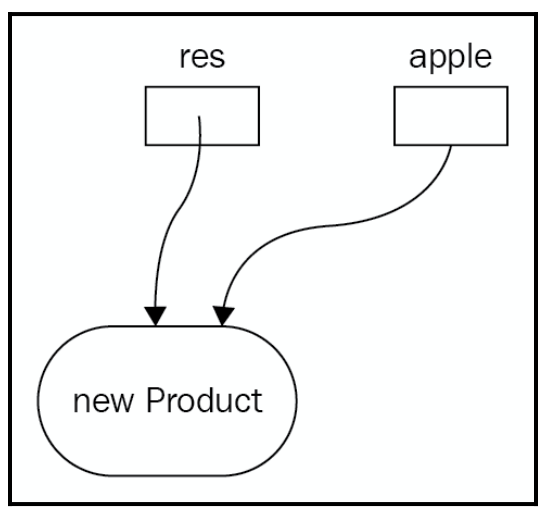
\includegraphics[width=0.3\textwidth]{content/Section-1/Chapter-5/13}
\end{center}

res和apple都拥有相同的资源。每当其中一个超出作用域(apple)时,底层资源就会释放,这使得另一个ResourceManager实例有一个悬空指针。当其他ResourceManager实例超出作用域时,将尝试删除该指针两次。通常,开发者知道他们在特定情况下需要哪种智能指针。这就是为什么C++提供了几种类型的智能指针,我们将进一步讨论这些类型。要在程序中使用它们,需要导入<memory>头文件。\par

\noindent\textbf{}\ \par
\textbf{std::unique\underline{ }ptr} \ \par
与我们前面实现的ResourceManager实例类似,std::unique\underline{ }ptr表示智能指针。例如,要使用这个智能指针管理Product对象: \par

\begin{lstlisting}[caption={}]
std::unique_ptr<Product> res{new Product};
res->set_name("Red apple");
// res will delete its acquired resource when goes out of scope
\end{lstlisting}

请注意我们如何访问Product成员函数set\underline{ }name。我们将res对象视为具有类型指针的对象。\par
unique\underline{ }ptr之所以命名为unique,因为提供了严格所有权的语义——它有义务销毁获得的对象,而且unique\underline{ }ptr不能复制,它没有复制构造函数或赋值操作符。这就是为什么它是所有权是严格的。当然,这并不意味着不能移动unique\underline{ }ptr。这种情况下,我们可以将所有权传递给另一个实例。 \par
智能指针的要求之一是轻量级。虽然unique\underline{ }ptr是一个包含多个成员函数的完整类,但它不会污染其他数据成员,只是一个封装了指向已分配对象的原始指针的容器。可以通过调用unique\underline{ }ptr的release()成员函数来访问这个原始指针,如下所示: \par

\begin{lstlisting}[caption={}]
Product* p = res.release();
// now we should delete p manually to deallocate memory
\end{lstlisting}

注意release()函数不调用delete操作符,只会归还所有权。调用release()函数后,unique\underline{ }ptr将不再拥有该资源。要重用已经拥有资源的unique\underline{ }ptr,应该使用reset()成员函数。为基础指针调用delete操作符,并重置智能指针,以供进一步使用。另一方面,如果想在不释放所有权的情况下获得基础对象,应该调用get(): \par

\begin{lstlisting}[caption={}]
std::unique_ptr<Product> up{new Product()};
Product* p = res.get();
// now p also points to the object managed by up
\end{lstlisting}

在以下场景中不能使用unique\underline{ }ptr类,因为它不能被复制: \par

\begin{lstlisting}[caption={}]
// Don't do this
void print_name(std::unique_ptr<Product> apple) {
	std::cout << apple->name();
}
std::unique_ptr<Product> res{new Product};
res->set_name("Red apple");
print_name(res); // bad code
res->set_price(0.42);
// ...
\end{lstlisting}

让我们继续C++中的下一个智能指针,它解决了将unique\underline{ }ptr传递给函数的问题。 \par

\noindent\textbf{}\ \par
\textbf{std::shared\underline{ }ptr和std::weak\underline{ }ptr} \ \par
我们需要提供共享所有权的智能指针,C++11中引入的std::shared\underline{ }ptr。实现具有共享所有权的智能指针比较困难,需要注意资源的正确重新分配。例如,当前面代码块中的print\underline{ }name()函数完成它的工作时,它的参数和局部对象将销毁。销毁智能指针会导致它所拥有的资源被适当地重新分配。智能指针如何知道该资源是否仍为另一个智能指针所拥有?一种解决方案是保存对资源的引用计数。shared\underline{ }ptr类做了同样的事情:它保留指向基础对象的指针的数量,并在使用计数变为0时删除它。因此,多个共享指针可以拥有同一个对象。 \par
现在,我们刚的例子应该这样改写: \par

\begin{lstlisting}[caption={}]
void print_name(std::shared_ptr<Product> apple) {
	std::cout << apple->name();
}
std::shared_ptr<Product> res{new Product};
res->set_name("Red apple");
print_name(res);
res->set_price(0.42);
// ...
\end{lstlisting}

调用print\underline{ }name()函数后,共享指针的使用计数增加1。当函数完成它的工作,但托管对象不会释放时,计数将减少1。这是因为res对象还没有超出作用域。让我们稍微修改一下示例,打印对共享对象的引用计数: \par

\begin{lstlisting}[caption={}]
void print_name(std::shared_ptr<Product> apple) {
	std::cout << apple.use_count() << " eyes on the " << apple->name();
}
std::shared_ptr<Product> res{new Product};
res->set_name("Red apple");
std::cout << res.use_count() << std::endl;
print_name(res);
std::cout << res.use_count() << std::endl;
res->set_price(0.42);
// ...
\end{lstlisting}

上述代码将会在屏幕上显示如下信息: \par

\begin{lstlisting}[caption={}]
1
2 eyes on the Red apple
1
\end{lstlisting}

当最后一个shared\underline{ }ptr超出作用域时,它也会销毁基础对象。然而,共享指针之间共享对象时应该小心。下面的代码显示了共享所有权的问题: \par

\begin{lstlisting}[caption={}]
std::shared_ptr<Product> ptr1{new Product()};
Product* temp = ptr1.get();
if (true) {
	std::shared_ptr<Product> ptr2{temp};
	ptr2->set_name("Apple of truth");
}
ptr1->set_name("Peach"); // danger!
\end{lstlisting}

ptr1和ptr2都指向同一个对象,但是它们不知道对方的存在。因此,当我们通过ptr2修改Product对象时,将影响ptr1。当ptr2超出作用域(在if语句之后)时,将销毁基础对象,该对象仍然由ptr1拥有。之所以会出现这种情况,是因为我们通过将原始的temp指针传递给ptr2,使其拥有对象。ptr1无法追踪。 \par
只能使用复制构造函数或std::shared\underline{ }ptr的赋值操作符共享所有权。这样,如果该对象正在被另一个shared\underline{ }ptr实例使用,就可以避免删除该对象。共享指针使用控制块实现共享所有权。每个共享指针包含两个指针,一个指向它管理的对象,另一个指向控制块。控制块表示动态分配的空间,其中包含资源的使用计数。它还包含其他几个对shared\underline{ }ptr至关重要的东西,例如:资源的分配器和删除器。我们将在下一节中介绍分配器。删除器通常是常规的删除操作符。 \par
控制块还包含弱引用的数量。这样做是因为所拥有的资源也可能指向一个弱指针。std::weak\underline{ }ptr是std::shared\underline{ }ptr的表示,它引用由shared\underline{ }ptr实例管理的对象,但不拥有该对象。weak\underline{ }ptr是一种访问和使用shared\underline{ }ptr拥有的资源,而不拥有它的方法。但是,有一种方法可以使用lock()成员函数将weak\underline{ }ptr实例转换为shared\underline{ }ptr。\par
unique\underline{ }ptr和shared\underline{ }ptr都可以用于管理动态分配的数组。模板参数必须正确指定: \par

\begin{lstlisting}[caption={}]
std::shared_ptr<int[]> sh_arr{new int[42]};
sh_arr[11] = 44;
\end{lstlisting}

要访问基础数组的元素,可以使用共享指针的[]操作符。另外,可以在动态多态性中使用智能指针。假设我们有如下的类层次结构: \par

\begin{lstlisting}[caption={}]
struct Base
{
	virtual void test() { std::cout << "Base::test()" << std::endl; }
};

struct Derived : Base
{
	void test() override { std::cout << "Derived::test()" << std::endl; }
};
\end{lstlisting}

以下代码按照预期工作,并将Derived::test()输出到屏幕:\par

\begin{lstlisting}[caption={}]
std::unique_ptr<Base> ptr = std::make_unique_default_init<Derived>();
ptr->test();
\end{lstlisting}

尽管智能指针的使用可能会破坏指针的美感,但建议使用智能指针可以避免内存泄漏。值得注意的是,用智能指针替换所有指针,无论是unique\underline{ }ptr指针还是shared\underline{ }ptr指针,都不能解决所有的内存泄漏问题。他们也有自己的缺点。考虑一种平衡的方法,或者更好的方法,在将智能指针应用于问题之前,彻底地了解问题和智能指针本身的细节。 \par
C++程序中管理内存是有代价的,我们讨论的最重要的事情是以适当地方式重新分配内存空间。语言不支持自动内存回收,但值得一提的是垃圾收集器。然而,要拥有一个完整的垃圾收集器,我们需要语言级的支持,但C++没有提供任何这些。让我们试着实现一个属于C++的垃圾收集器。 \par

\noindent\textbf{}\ \par
\textbf{垃圾收集} \ \par
垃圾收集器是一个单独的模块,通常合并在可解释语言的运行时环境中。C\#和Java都有垃圾收集器,这使开发者的工作变得容易得多。垃圾收集器跟踪代码中所有的对象分配,并在它们不再使用时释放它们。称为垃圾收集器,因为它在使用内存资源后删除内存资源:收集开发者留下的垃圾。\par
据说C++程序员不会留下垃圾,这就是为什么语言不支持垃圾收集器的原因。尽管开发者倾向于为语言进行辩护,说它没有垃圾收集器,因为它是一种快速的语言,但事实是有垃圾收集器也不影响速度。 \par
像C\#这样的语言,将程序编译成中间字节码表示,然后由运行时环境解释和执行。垃圾收集器是环境的一部分,并积极跟踪所有对象分配。它是一种复杂的动物,它会尽力在合理的时间内管理内存。下图描述了一个典型的运行时环境,在垃圾收集器的监督下分配内存: \par

\begin{center}
	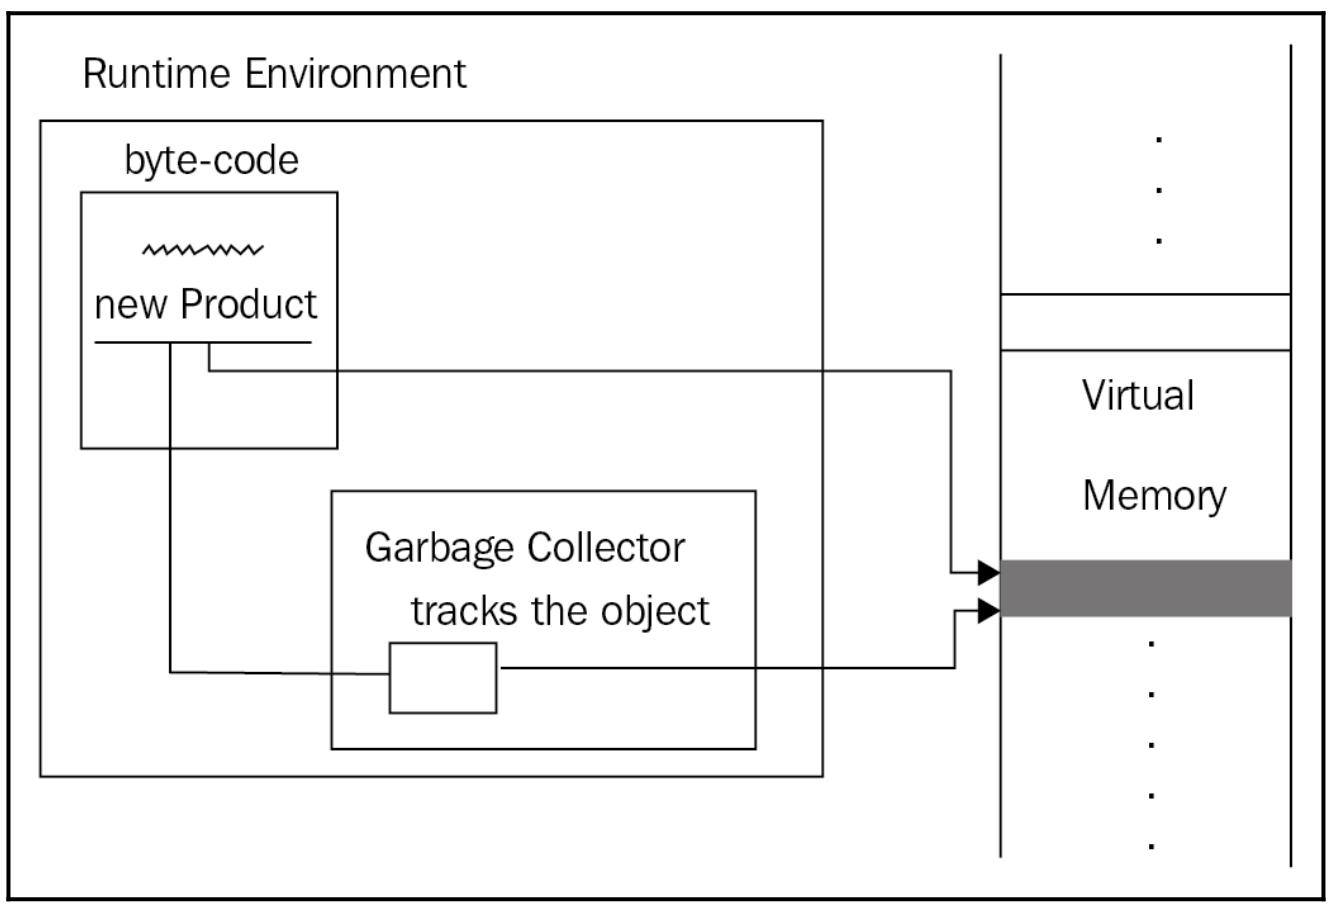
\includegraphics[width=0.6\textwidth]{content/Section-1/Chapter-5/14}
\end{center}

C++中使用智能指针,也可以手动调用delete操作符来释放内存空间。智能指针只获取对象,并在对象超出作用域时删除对象。关键的是,即使智能指针引入了一些半自动行为,仍然像开发者没有忘记在代码的指定点释放资源一样工作。垃圾收集器会自动执行,并且通常使用单独的执行线程。它尽量不减慢实际程序的执行速度。\par
一些垃圾收集实现技术包括根据对象的生存期对其进行分类,分类使垃圾收集器访问对象,并在对象不再使用时释放内存空间。为了使这个进程更快,应该访问生命周期较短的对象比访问生命周期较长的对象更频繁。以下面的代码为例: \par

\begin{lstlisting}[caption={}]
struct Garbage {
	char ch;
	int i;
};

void foo() {
	Garbage* g1 = new Garbage();
	if (true) {
		Garbage* g2 = new Garbage();
	}
}

int main() {
	static Garbage* g3 = new Garbage();
}
\end{lstlisting}

如果C++有一个垃圾收集器,那么对象g1、g2和g3将在程序执行的不同时间段删除。如果垃圾收集器根据生命周期进行分类,那么g2的生命周期将是最短的,并且应该首先访问它以释放它。 \par
真正在C++中实现垃圾收集器,应该让它成为程序的一部分。垃圾收集器首先应该负责分配内存来跟踪和删除它: \par

\begin{lstlisting}[caption={}]
class GarbageCollector {
public:
	template <typename T>
	static T* allocate() {
		T* ptr{new T()};
		objects_[ptr] = true;
		return ptr;
	}
	static void deallocate(T* p) {
		if (objects_[p]) {
			objects_[p] = false;
			delete p;
		}
	}
private:
	std::unordered_map<T*, bool> objects_;
};
\end{lstlisting}

前面的类跟踪通过静态allocate()函数分配的对象。如果对象正在使用,则通过deallocate()函数删除该对象。下面是如何使用垃圾收集器: \par

\begin{lstlisting}[caption={}]
int* ptr = GarbageCollector::allocate<int>();
*ptr = 42;
GarbageCollector::deallocate(ptr);
\end{lstlisting}

这个类使内存管理比智能指针更难一些。基本上,在C++中不需要实现垃圾收集器,因为智能指针可以处理几乎所有与自动内存回收有关的场景。 \par
但是,让我们来看看垃圾收集器正确地释放指针所指向空间的技巧。前面最简单的实现中,我们跟踪了提供给用户的所有指针。每个指针都指向堆上的某个空间,这些空间应该在程序执行的某个点释放。GarbageCollector中将使用标准的delete操作符。问题是,它怎么知道应该释放多少字节?看看下面的例子: \par

\begin{lstlisting}[caption={}]
Student* ptr = new Student;
int* ip = new int{42};
// do something with ptr and ip
delete ptr;
delete ip;
\end{lstlisting}

假设一个Student实例占用40个字节的内存,一个整数占用4个字节。我们应该以某种方式将该信息传递给delete操作符。在前面的代码中,我们删除了ptr和ip,它们都指向不同大小的内存空间。那么它如何知道在ptr的情况下40个字节应该标记为空闲,而在ip的情况下4个字节应该被标记为空闲?这个问题有不止一个解决方案,所以让我们看看其中一个。\par
无论何时分配内存,new操作符都会将分配的内存大小置于实际内存空间之前,如下图所示: \par

\begin{center}
	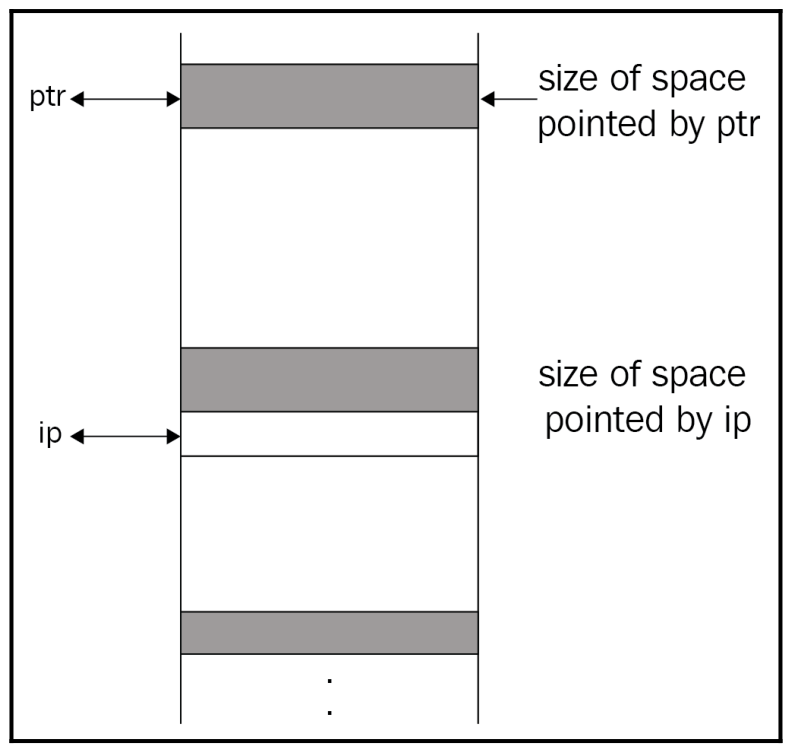
\includegraphics[width=0.6\textwidth]{content/Section-1/Chapter-5/15}
\end{center}

然后,该信息由delete操作符使用,该操作符通过读取放置在内存空间之前的相应字节,来获取内存空间的大小。C++最关心的问题是管理数据集合的内存。STL容器,如std::vector和std::list,有不同的处理内存的模型。默认情况下,容器有一个指定的内存分配器,用于处理容器元素的内存分配和回收。 \par

\noindent\textbf{}\ \par
\textbf{使用分配器} \ \par
分配器背后的思想是为容器内存管理提供控制。简单地说,分配器是C++容器的高级垃圾收集器。尽管在容器内存管理的范围内讨论分配器,但肯定可以将这个想法扩展到通用的垃圾收集器。本节的开始部分,实现了一个设计糟糕的垃圾收集器。检查分配器时,会发现设计糟糕的garbagcollector类和C++中的默认分配器之间有很多相似之处。在<memory>中定义的默认分配器有两个基本函数——allocate()和deallocate()。allocate()函数的定义如下: \par

\begin{lstlisting}[caption={}]
[[nodiscard]] constexpr T* allocate(std::size_t num);
\end{lstlisting}

allocate()函数为类型为T的num对象获取空间。请注意[[nodiscard]]属性——它意味着返回值不应该被调用者丢弃。否则,编译器将报出警告消息。 \par
使用分配器,为5个整数获取空间: \par

\begin{lstlisting}[caption={}]
import <memory>;
int main()
{
	std::allocator<int> IntAlloc;
	int* ptr = IntAlloc.allocate(5);
	// construct an integer at the second position
	std::allocator_traits<IntAlloc>::construct(IntAlloc, ptr + 1, 42);
	IntAlloc.deallocate(ptr, 5); // deallocate all
}
\end{lstlisting}

注意,我们是如何使用std::allocator\underline{ }traits在已分配的空间中构造对象的。 \par
deallocate()函数的定义如下: \par

\begin{lstlisting}[caption={}]
constexpr void deallocate(T* p, std::size_t n)
\end{lstlisting}

前面的代码片段中,我们通过传递allocate()函数返回的指针来使用deallocate()函数。\par
可能不会在项目中直接使用分配器,但是每当需要内存管理的自定义行为时,使用现有的或引入新的分配器可能会有帮助。STL容器使用分配器主要是因为在结构和行为上的不同,这导致需要对内存分配和回收有专门的行为。我们将在下一章更详细地讨论STL容器。 \par

\noindent\textbf{}\ \par
\textbf{总结} \ \par
C\#等语言中提供了垃圾收集器。它们与用户程序并行工作,并试图在程序看起来有效时在程序结束后进行清理。不能在C++中做同样的事情,我们所能实现的就是在程序中直接实现垃圾收集器,提供一种半自动的方式来释放使用过的内存资源。自C++11以来,语言中引入的智能指针,可以适当地涵盖了这种机制。 \par
内存管理是每个计算机程序的关键组成部分之一。程序应该能够在其执行期间动态地请求内存。优秀的开发者理解内存管理的内部细节,这有助于他们设计和实现性能更高的应用程序。虽然手动内存管理是一种优势,在大型应用程序中,往往会变得很痛苦。本章中,我们已经学习了如何使用智能指针来避免错误和处理内存回收。有了这些基本的了解,就能增强设计避免内存泄漏的程序的信心。 \par
下一章中,我们将学习STL,关注数据结构和算法,并深入研究它们的STL实现。除了比较数据结构和算法之外,还将介绍C++20中一个值得注意的新特性:概念。 \par

\noindent\textbf{}\ \par
\textbf{问题} \ \par
\begin{enumerate}
	\item 解释计算机内存。
	\item 什么是虚拟内存?
	\item 哪些是用于内存分配和回收的操作符?
	\item delete和delete[]有什么区别?
	\item 什么是垃圾收集器?为什么C++不支持垃圾收集?
\end{enumerate}

\noindent\textbf{}\ \par
\textbf{扩展阅读} \ \par
更多信息,请参阅以下链接: \par

\begin{itemize}
	\item What every programmer should know about memory, by Ulrich Drepper, at  https:/​/​people.​freebsd.​org/​~lstewart/​articles/​cpumemory.​pdf
	\item Code: The hidden language of computer hardware and software, by Charles Petzold, at  https:/​/​www.​amazon.​com/​Code-​Language-​Computer-​Hardware-	Software/​dp/​0735611319/​
\end{itemize}

\newpage



